\documentclass[conference]{IEEEtran}

\usepackage[utf8]{inputenc}
\usepackage{hyperref} % Hyperlinks
\usepackage{indentfirst} % Indent first line section
\usepackage{enumerate} % Ordered list
\usepackage{multibib} % Multiple bibliographies
\usepackage{graphicx} % Allows for figures
\graphicspath{ {./.assets/images/} }

\newcites{SLR}{Systematic Review References}

\title{Refactoring-assisted migration of monoliths to microservices}
\author{Breno Salles} \date{January 2023}

\begin{document}

\maketitle

\begin{abstract}

  Lorem rem amet nesciunt voluptate ullam sapiente. Optio nemo alias nesciunt
  illo minima. Modi deleniti repellendus sint tempora quidem Eum quibusdam
  recusandae nostrum exercitationem dolores. Cum harum sapiente reiciendis
  inventore delectus neque! Deserunt unde hic sunt vel culpa Totam in corporis
  qui corrupti at magnam Dignissimos tempore quibusdam ipsa nobis illum Quis
  adipisci ex incidunt fuga nam sequi architecto adipisci facere Aut quam nulla
  cum sed expedita accusamus! Qui inventore molestias inventore quo officiis
  quibusdam, repellendus Facere rem a magnam aliquid doloribus distinctio
  distinctio? Labore dolorum quos veritatis neque culpa Saepe vero placeat qui
  odit excepturi Fugit laborum a eos

\end{abstract}

\section{Introduction}

Microservices is an architectural style that evolved from Service Oriented
Architecture (SOA). Just like SOA, microservices are a response to monolithic
architecture. The main contrasts are that, while monolithic applications are
software systems with a single, integrated codebase that includes all necessary
components and features \cite{kazanavivcius2019migrating}, microservices tend
to be separated and loosely coupled \cite{newman2021building}, and also that
while monoliths tend to be easier to develop they may scale poorly and are
harder do maintain when compared to microservices \cite{newman2019monolith}.

Microservices are increasingly being used in the development of modern
applications, particularly in the areas of cloud computing and DevOps
\cite{ren2018migrating}. Many organizations, including large enterprises and
startups, are adopting microservices as a way to build and deploy applications
more quickly and efficiently \cite{richardson-microservices}. Microservices are
particularly well-suited to distributed, cloud-based environments, where they
can take advantage of the flexibility and scalability of the cloud
\cite{fowler-microservices-prerequisites}. This type of architecture is already
being applied in multiple well known companies, like Uber, Netflix, Ebay
\cite{microservices-users} and also being followed by the rest of the herd when compared to monolith architecture \cite{taibi2017processes}.

Refactoring from monoliths to microservices is a heavily debated topic both in
the academic world and the industry. The main takes from this debate is that
refactoring is difficult and time consuming if a proper ways of migration are
chosen. To help fight this, some tools were developed that help with the
refactor \cite{brito2021identification} \cite{kalia2021mono2micro}
\cite{freitas2021refactoring}, but in a world with more and more data and
information, having a single place where architects, engineers and developers
can find and use all these and future tools can be considered utopia.

The goal of this study is to structurally analyse the state of the art in
regards of migration of monolithic applications to microservices architectural
style, mainly how tools are helping architects, engineers and developers in
this migration, and how automated they are. Furthermore, in the following
thesis, the purpose is to develop a tool which aims to aggregate existing tools
into a single platform, as well as provide the means to extend and incorporate
new tools. This tool will offer a convenient and comprehensive way to access
and use a variety of tools that help on the refactor from monolith to
microservices.

To achieve this, the guidelines presented by Kitchenham and Charters
\citeSLR{kitchenham2007guidelines} were taken into account while performing a
systematic literature review. The research protocol was defined at first and then followed to ensure all results could be reproduced.

According to Kitchenham and Charters \citeSLR{kitchenham2007guidelines},
research questions should be specified as they will direct the entire review
methodology. The research questions formulated are as follows:

\emph{
  \begin{enumerate}[{RQ}1.]
    \item What tools already exist that aid in the migration process of
      monoliths to microservices?
    \begin{enumerate}[{RQ1.}1.]
      \item How do they take the monolith as input?
      \item How do they produce the microservice as output?
      \item Are they bound to a specific language?
    \end{enumerate}
    \item How can an aggregator of those tools help architects, engineers
      and developers in their microservice migration?
  \end{enumerate}
}

\section{Background}

To give readers a foundational understanding of microservice architecture and
its key features, we will provide a brief overview of microservices and
contrast them with traditional monolithic applications. This will allow readers
to clearly understand the differences between the two architectures.

\subsection{Monoliths}

Monolithic applications are software systems that are designed as a single,
self-contained unit. In other words, monolithic applications are composed of a
single, integrated codebase that includes all of the necessary components and
features for the application to run \cite{kazanavivcius2019migrating}. This
means that all of the different parts of the application, such as the user
interface, business logic, and database access, are all contained within a
single codebase and are not modularized or separated into distinct components.

Monolithic architecture is a traditional approach to software development that
has been widely used for many years. It is generally characterized by a strong
emphasis on simplicity and ease of development. However, monolithic
applications can also be more difficult to maintain and update, as changes to
one part of the codebase can have unintended consequences on other parts of the
system. This can make it challenging to introduce new features or make changes
to the application without significant testing and debugging
\cite{kazanavivcius2019migrating}.

Despite these challenges, monolithic applications are still widely used in many
contexts due to their simplicity and ease of development. They are particularly
well-suited for small to medium-sized applications that do not require a high
level of modularity or separation of concerns.

\subsection{Microservices}

Microservices is an architectural style that structures an application as a
collection of loosely coupled services \cite{newman2021building}. This means
that each microservice is a self-contained unit of functionality, which
communicates with other microservices through well-defined interfaces,
typically using a lightweight messaging protocol such as HTTP
\cite{fowler-microservices}.

One key benefit of this approach is that it allows for greater flexibility and
scalability \cite{newman2019monolith}. Because each microservice is independent
and modular, it can be modified and deployed independently of the other
services in the application. This can make it easier to make changes to the
system, as it is not necessary to redeploy the entire application every time a
change is made. In addition, the modular nature of microservices allows for
easier scaling, as individual services can be scaled up or down as needed to
meet changing demand
\cite{newman2019monolith}\cite{newman2021building}\cite{fowler-microservices}.

Another advantage of microservices is that they can be developed and maintained
by small, autonomous teams \cite{chen2018microservices}. This can be beneficial
for organizations with a large codebase or a distributed development team, as
it allows for more focused development and faster deployment of changes
\cite{nadareishvili2016microservice}.

However, there are also challenges to consider when adopting a microservices
architecture \cite{fowler-microservices-tradeoffs}. One challenge is the added
complexity of managing a distributed system, as there may be a larger number of
moving parts to monitor and troubleshoot \cite{newman2021building}. In
addition, the communication between microservices can add latency to the
system, which may impact the performance of the overall application
\cite{fowler-microservices-tradeoffs} \cite{pautasso2017microservices}.

Overall, microservices can be an effective way to structure an application,
particularly for large, complex systems that require a high degree of
flexibility and scalability \cite{newman2021building}. However, it is important
to carefully evaluate the trade-offs and consider whether the benefits of a
microservices architecture are worth the added complexity
\cite{fowler-microservices-tradeoffs}.

\subsection{Refactoring}

Refactoring is the process of modifying the internal structure of an existing
codebase without changing its external behavior \cite{becker1999refactoring}.
When migrating from a monolithic architecture to a microservices architecture,
it may be necessary to refactor the existing codebase in order to break it up
into independent microservices. This can be a complex and time-consuming
process, particularly for large, complex systems \cite{newman2019monolith}.

There are several factors to consider when refactoring an existing codebase for
a microservices architecture \cite{newman2019monolith}. One challenge is
ensuring that the code is modular and loosely coupled, so that it can be
developed and deployed independently as a microservice. This may require
restructuring the code, introducing new abstractions and interfaces, and
potentially even rewriting parts of the code.

Another challenge is preserving the existing functionality of the application
while making changes to the codebase. It is important to carefully plan and
test the refactoring process to ensure that the application continues to work
as expected after the changes are made.

Overall, refactoring an existing codebase for a microservices architecture can
be a significant undertaking, and it is important to carefully evaluate the
resources and time required to complete the process \cite{newman2019monolith}.

\section{Systematic Literature Review}

A systematic literature review is a type of review that aims to identify,
evaluate, and summarize the results of all studies that address a specific
research question or topic \citeSLR{kitchenham2007guidelines}
\citeSLR{kitchenham2009systematic} \citeSLR{gough2017introduction}. It involves
following a specific methodology to identify, analyze, and interpret all
relevant evidence related to the research question being addressed. The purpose
of a systematic literature review is to provide a comprehensive and up-to-date
overview of the current state of knowledge on a specific research question or
topic. It is a critical appraisal of the existing research, and it can help
identify gaps in the literature and inform future research directions
\citeSLR{kitchenham2007guidelines}.

As per Kitchenham and Charters guidelines \citeSLR{kitchenham2007guidelines}, a
systematic literature review (SLR) involves three phases: planning, conducting,
and reporting. The planning phase involves establishing the review protocol
based on the research questions and the need for the review. The conducting
phase involves selecting primary studies and applying the criteria established
in the review protocol to analyze them. Finally, the reporting phase involves
the creation of the report. These guidelines were loosely followed in the
development of this review.

\subsection{Research Methodology} \label{sub:research-methodology}



To address the research questions posed in the Introduction, the appropriate
research methods were utilized.

\subsubsection{Data sources and search strategy} \label{sub:search-strategy}

To access relevant research and information in this field, it is advisable to
search several databases that specialise in scientific literature. Table
\ref{tab:databases} presents a list of several such databases, including the
ACM Digital Library, Science Direct, IEEE Xplore, Wiley, Springer Link,
Engineering Village, and Google Scholar. These databases contain a wealth of
knowledge and resources, including journal articles, conference proceedings,
technical reports, and more, which can be useful for staying up to date on the
latest developments in this field.

\begin{table}[!htb] \caption{Databases} \label{tab:databases}
  \begin{center}
    \begin{tabular}[c]{l|l|l} \textbf{ID} & \textbf{Search Engine} &
      \textbf{Website} \\
      \hline DB.1 & ACM Digital Library & \url{https://dl.acm.org/} \\
      \hline DB.2 & IEEE Xplore & \url{https://ieeexplore.ieee.org/} \\
      \hline DB.3 & Springer Link & \url{https://link.springer.com/} \\
      \hline DB.4 & Wiley & \url{https://onlinelibrary.wiley.com/} \\
      \hline DB.5 & Science Direct & \url{https://www.sciencedirect.com/} \\
      \hline DB.6 & Engineering Village &
      \url{https://www.engineeringvillage.com/} \\
      \hline DB.7 & Google Scholar & \url{https://scholar.google.com/} \\
    \end{tabular}
  \end{center}
\end{table}


% TODO: Aqui estava a pensar introduzir a palha a explicar o que são por alto

To ensure a thorough and comprehensive search for relevant publications in this
field, we will utilize a breadth first search approach. This method involves
starting with a specific query string and selecting relevant publications from
a given database. We will then use a technique called snowballing to expand the
search and locate additional relevant publications. Snowballing involves
searching for citations and publications that are related to the initially
selected publications.

There are two types of snowballing that we will employ in this search: forward
snowballing and backward snowballing. Forward snowballing involves searching
for citations and publications using Google Scholar for the initially selected
publications. This process can be repeated multiple times, with each iteration
referred to as a level of snowballing. For the purpose of this search, we will
perform two levels of forward snowballing, in which we extract the references
of the initially selected publications (level one) and then select the
references of those references (level two).

Backward snowballing involves searching for publications that have cited the
initially selected publications. This technique can also be repeated multiple
times, but for the purpose of this search, we will only perform one level of
backward snowballing. This will include all previous publications found during
the forward snowballing step.

By utilizing both forward and backward snowballing techniques, we aim to cast a
wide net and identify as many relevant publications as possible.

After completing the search for relevant publications in a given database using
the specified query string, we will move on to the next database. This approach
is advantageous because it allows us to efficiently locate relevant
publications while minimizing the number of duplicates that are analyzed. By
searching multiple databases and using snowballing techniques, we can identify
a large number of relevant publications and eliminate the need to analyze many
of them in subsequent iterations.

To identify relevant publications for this research, we will utilize a range of
keywords related to the topic of microservices. These keywords will include
various phrases and terms used to describe microservices. As for the practices
that may help identification of microservices, keywords that help this
architectural refactoring should be included, things like ``migration",
``refactor", ``identification". It could also be useful to use ``monolith" (and
all its possible synonyms) to be the comparison against ``microservices",
although this can result in some extra publications not related to
microservices but instead related to ``service oriented architecture". An
expected outcome or conclusion of the publication could be included,
``approach" or even ``tool".

\begin{table}[!htb] \caption{Keywords} \label{tab:keywords}
  \begin{center}
    \begin{tabular}[c]{p{7em}|p{13em}} {\textbf{Focus}} & microservices \\
      \hline \textbf{Refactoring} & {migration, decomposition, identify, refactor, evolve, discover, transition } \\
      \hline \textbf{Target} & monolith \\
      \hline \textbf{Outcome} & approach, tool \\
    \end{tabular}
  \end{center}
\end{table}


\subsubsection{Selection Criteria} \label{sub:selection-criteria}

In order to filter the publications, the title and the abstract will be
analysed and should mention some at least one of:

\begin{enumerate}[{IC}1.]
  \item A tool that automates process of migration of monoliths to
    microservices.
  \item Identification of microservices from monolith systems.
  \item Analysis of tools or approaches for migrating from monoliths to
    microservices.
\end{enumerate}

In cases of ambigous conclusions, further inspection of the publication may
be done. When this happens, and if relevant publications apply, conclusions
should also be taken into account.

As for more pratical approach for exclusion of publications, the criteria
will be:

\begin{enumerate}[{EC}1.]
  \item Publications that are not written in English or Portuguese.
  \item For Portuguese publications, English must be the language used in
    the
  \item Publication is not accessible.
\end{enumerate}

\subsection{Research Results}

In the first iteration of the review, the main purpose was figuring out how
many tools exist that were able to solve this research question or, at the
very least, help partially with it. In order to do this, one could not be
limited to tools that are documented in academic databases therefore, in
addition to the databases mentioned in Table \ref{tab:databases},
\href{https://github.com}{GitHub}, \href{https://gitlab.com}{GitLab} and
even \href{https://duckduckgo.org}{DuckDuckGo} were searched for, even
though they do not represent a scientific search engine.

By using some keywords mentioned in Table \ref{tab:keywords} we created an
initial trial query:

\begin{center}
  \emph{("microservice" OR "micro-service") AND ("migration" OR
  "identification") AND ("monolithic" OR "monolith") AND ("tool")}
\end{center}


The query was then applied to DB.1, DB.2 and DB.3 and after applying the
selection criteria mentioned in subsection \ref{sub:selection-criteria},
results were gathered and are presented in Table \ref{tab:tool-search}.

\begin{table}[!htb] \caption{Tool Search} \label{tab:tool-search}
  \begin{center}
    \begin{tabular}[c]{p{5.5em}|p{5em}|p{5em}} \textbf{Database} &
      \textbf{Total\newline number\newline of results} &
      \textbf{Extracted\newline Results} \\
      \hline DB.1 & {118} & {3} \\
      \hline DB.2 & {4} & {0} \\
      \hline DB.3 & {658} & {3} \\
    \end{tabular}
  \end{center}
\end{table}

As for the not so scientific search, the query would be essentilly typed into
their respective search engine and the results gathered are present in Table
\ref{tab:search-engine-tool-search}.

\begin{table}[!htb] \caption{Search Engine Tool Search}
  \label{tab:search-engine-tool-search}
  \begin{center}
    \begin{tabular}[c]{p{5.5em}|p{10em}|p{4em}|p{5em}}
      \textbf{Search\newline Engine} &
      \textbf{Query} &
      \textbf{Total\newline number\newline of results} &
      \textbf{Extracted\newline Results} \\
      \hline
        GitHub &
        \url{https://github.com/search?q=monolith+to+microservice} &
        {745} &
        {4} \\
      \hline
        GitLab &
        \url{https://gitlab.com/search?search=monolith\%20to\%20microservice} &
        {0} &
        {0} \\
      \hline
        DuckDuckGo &
        \url{https://duckduckgo.com/?q=monolith+to+microservices+tool} &
        {Infinity} &
        {2} \\
    \end{tabular}
  \end{center}
\end{table}

Through this search process, we can also trace the references used in these
publications to determine if the tools described were based on previous work,
but only implemented a specific approach. This will help us to understand the
context and origins of these tools and how they fit into the broader landscape
of research in this area.

During the second iteration of the review process, we focused on locating
publications that describe alternative approaches for migrating from monolithic
to microservices architectures that may not have been implemented in practice.
This allowed us to gain a deeper understanding of the current state of the art
in this area, identify any gaps or areas where further research is needed, and
determine what can be improved upon. This information will be useful in guiding
the development of our tool and abstraction.

As this was the beginning of a new iteration of the review process, the results
of the previous ``test run" were not considered when extracting literature.
Only after this iteration was completed did we incorporate the previously
analysed literature and exclude it from further analysis to avoid duplication
of effort. This allowed us to focus on identifying new and potentially relevant
publications for our purposes.

Relying on the keywords identified in Table \ref{tab:keywords}, the following
query was tried:

\begin{center}
  \emph{(microservice* OR micro?service*) AND (migrat* OR identif*) AND
  (monolith*) AND (migrat* NEAR/2 (process* OR approach*))}
\end{center}

With this, we then proceed to apply the query and search the first database. As
shown in Table \ref{tab:db1-search}, from four hundred and fifty results, only
twelve passed the selection criteria defined in section
\ref{sub:selection-criteria}.

\begin{table}[!htb] \caption{DB.1 Results} \label{tab:db1-search}
  \begin{center}
    \begin{tabular}[c]{p{5em}|p{5em}} \textbf{Total\newline number\newline of
      results} & \textbf{Extracted\newline New Results} \\
      \hline{450} & {12} \\
    \end{tabular}
  \end{center}
\end{table}

After reviewing the references of the identified papers and applying forward
and backward snowballing techniques, we were able to locate additional related
publications and expand the scope of our search as demonstrated in Table
\ref{tab:db1-snowballing}. This helped us to increase the number of relevant
publications that we were able to consider in the next steps of the process.

\begin{table}[!htb] \caption{DB.1 Snowballing Results} \label{tab:db1-snowballing}
  \begin{center}
    \begin{tabular}[c]{p{8em}|p{8em}|p{8em}}
      \textbf{1st Forward} &
      \textbf{2nd Forward} &
      \textbf{Backward} \\
      \hline{23} &
      {2} &
      {45} \\
    \end{tabular}
  \end{center}
\end{table}

After a certain point, we found that the publications located through the
snowballing approach were no longer adding significant value to our overall
understanding of the topic. As a result, we decided to apply the search query
to the remaining databases. In some instances, the query produced more than two
thousand results, which would have been impractical to analyse within the given
timeframe. Therefore, we modified the query to focus only on the titles and
abstracts of the publications. The revised query that we used is as follows:

\begin{center}
  \emph{(microservice* OR "micro-service") AND (migrat* OR decompos* OR
  identif* OR refactor* OR evolv* OR extract* OR discover* OR transition*)}
\end{center}

\begin{table}[!htb] \caption{Remaining DB Results} \label{tab:other-db-search}
  \begin{center}
    \begin{tabular}[c]{p{5em}|p{5em}|p{5em}}
      \textbf{Database} &
      \textbf{Total\newline number\newline of results} &
      \textbf{Extracted\newline New Results} \\
      \hline {DB.5 - 1st} & {21} & {1} \\
      \hline {DB.5 - 2nd} & {0} & {0} \\
      \hline {DB.4} & {9} & {3} \\
      \hline {DB.6} & {114} & {12} \\
      \hline {DB.3} & {20} & {0} \\
      \hline {DB.2} & {0} & {0} \\
    \end{tabular}
  \end{center}
\end{table}

In the case of Science Direct, as presented in Table \ref{tab:other-db-search},
two queries were done. The main reason for this is that Science Direct is
limited to 7 \textit{OR} conditions, therefore it was necessary to split it
into two queries where it does not affect the general condition. In the
specific case, the \textit{``evolv"} keyword was moved into a separate query.
Also, Scince Direct automatically accepts truncations without using the
\textit{``*"} char.

\begin{enumerate}
  \item \emph{(microservice OR "micro-service") AND ( migrat OR decompos OR
    identif OR refactor OR extract OR discover OR transition)}
  \item \emph{(microservice OR "micro-service") AND (evolv)}
\end{enumerate}


After iterating over the results and reviewing the references of the newly
found publications, we did not identify any additional publications that were
worth including in the final list. This marked the end of our general search
for relevant publications.

\subsection{Publications Grouping}

Given the large number of publications that were identified as potential
candidates for further analysis, it was necessary to further narrow down the
list to a more manageable size. To accomplish this, we employed a
categorization approach in order to better organize and prioritize the
publications for later selection. This allowed us to more efficiently select
and analyze the most relevant publications for our purposes. Through this
process, we arrived at four main categories into which we could place each
publication:

\begin{itemize}
  \item The \textbf{approach} used for identifying microservices from monoliths.
  \begin{itemize}
    \item \textit{Data flow}.
    \item \textit{Dependency analysis}.
    \item \textit{Execution log}.
    \item \textit{etc}.
  \end{itemize}
  \item The current \textbf{status} of the publication.
  \begin{itemize}
    \item It only explains the \textit{method} at a high level.
    \item Has implementation details with the \textit{algorithm} on how to identify.
    \item Already has a working \textit{tool}.
  \end{itemize}
  \item The \textbf{language} in which that it targets.
  \begin{itemize}
    \item \textit{Java}.
    \item \textit{Cpp}.
    \item \textit{C}.
    \item \textit{Language Agnostic}.
    \item \textit{etc}.
  \end{itemize}
\end{itemize}

% \begin{table}[!htb] \caption{Approach grouping}
%   \begin{center}
%     \begin{tabular}[c]{p{8em}|p{4em}}
%       \textbf{Approach} &
%       \textbf{Amount} \\
%       \hline Static analysis & {13} \\
%       \hline Model based & {9} \\
%       \hline Dependency analysis  & {7} \\
%       \hline Domain analysis  & {6} \\
%       \hline Data flow  & {6} \\
%       \hline Data & {5} \\
%       \hline Cohesion & {4} \\
%       \hline Multiple & {4} \\
%     \end{tabular}
%   \end{center}
% \end{table}

\subsection{Selected Work}

\section{Tool Design}

As of the time of writing this paper, the design of the proposed tool is not
yet finalized. We have only developed initial ideas about how we will approach
the problem and have created a sketch of the proposed tool architecture, which
is shown in Figure \ref{fig:tool-architecture}.

\begin{figure}[!htb]
  \caption{Candidate tool architecture}
  \label{fig:tool-architecture}
  \centering
  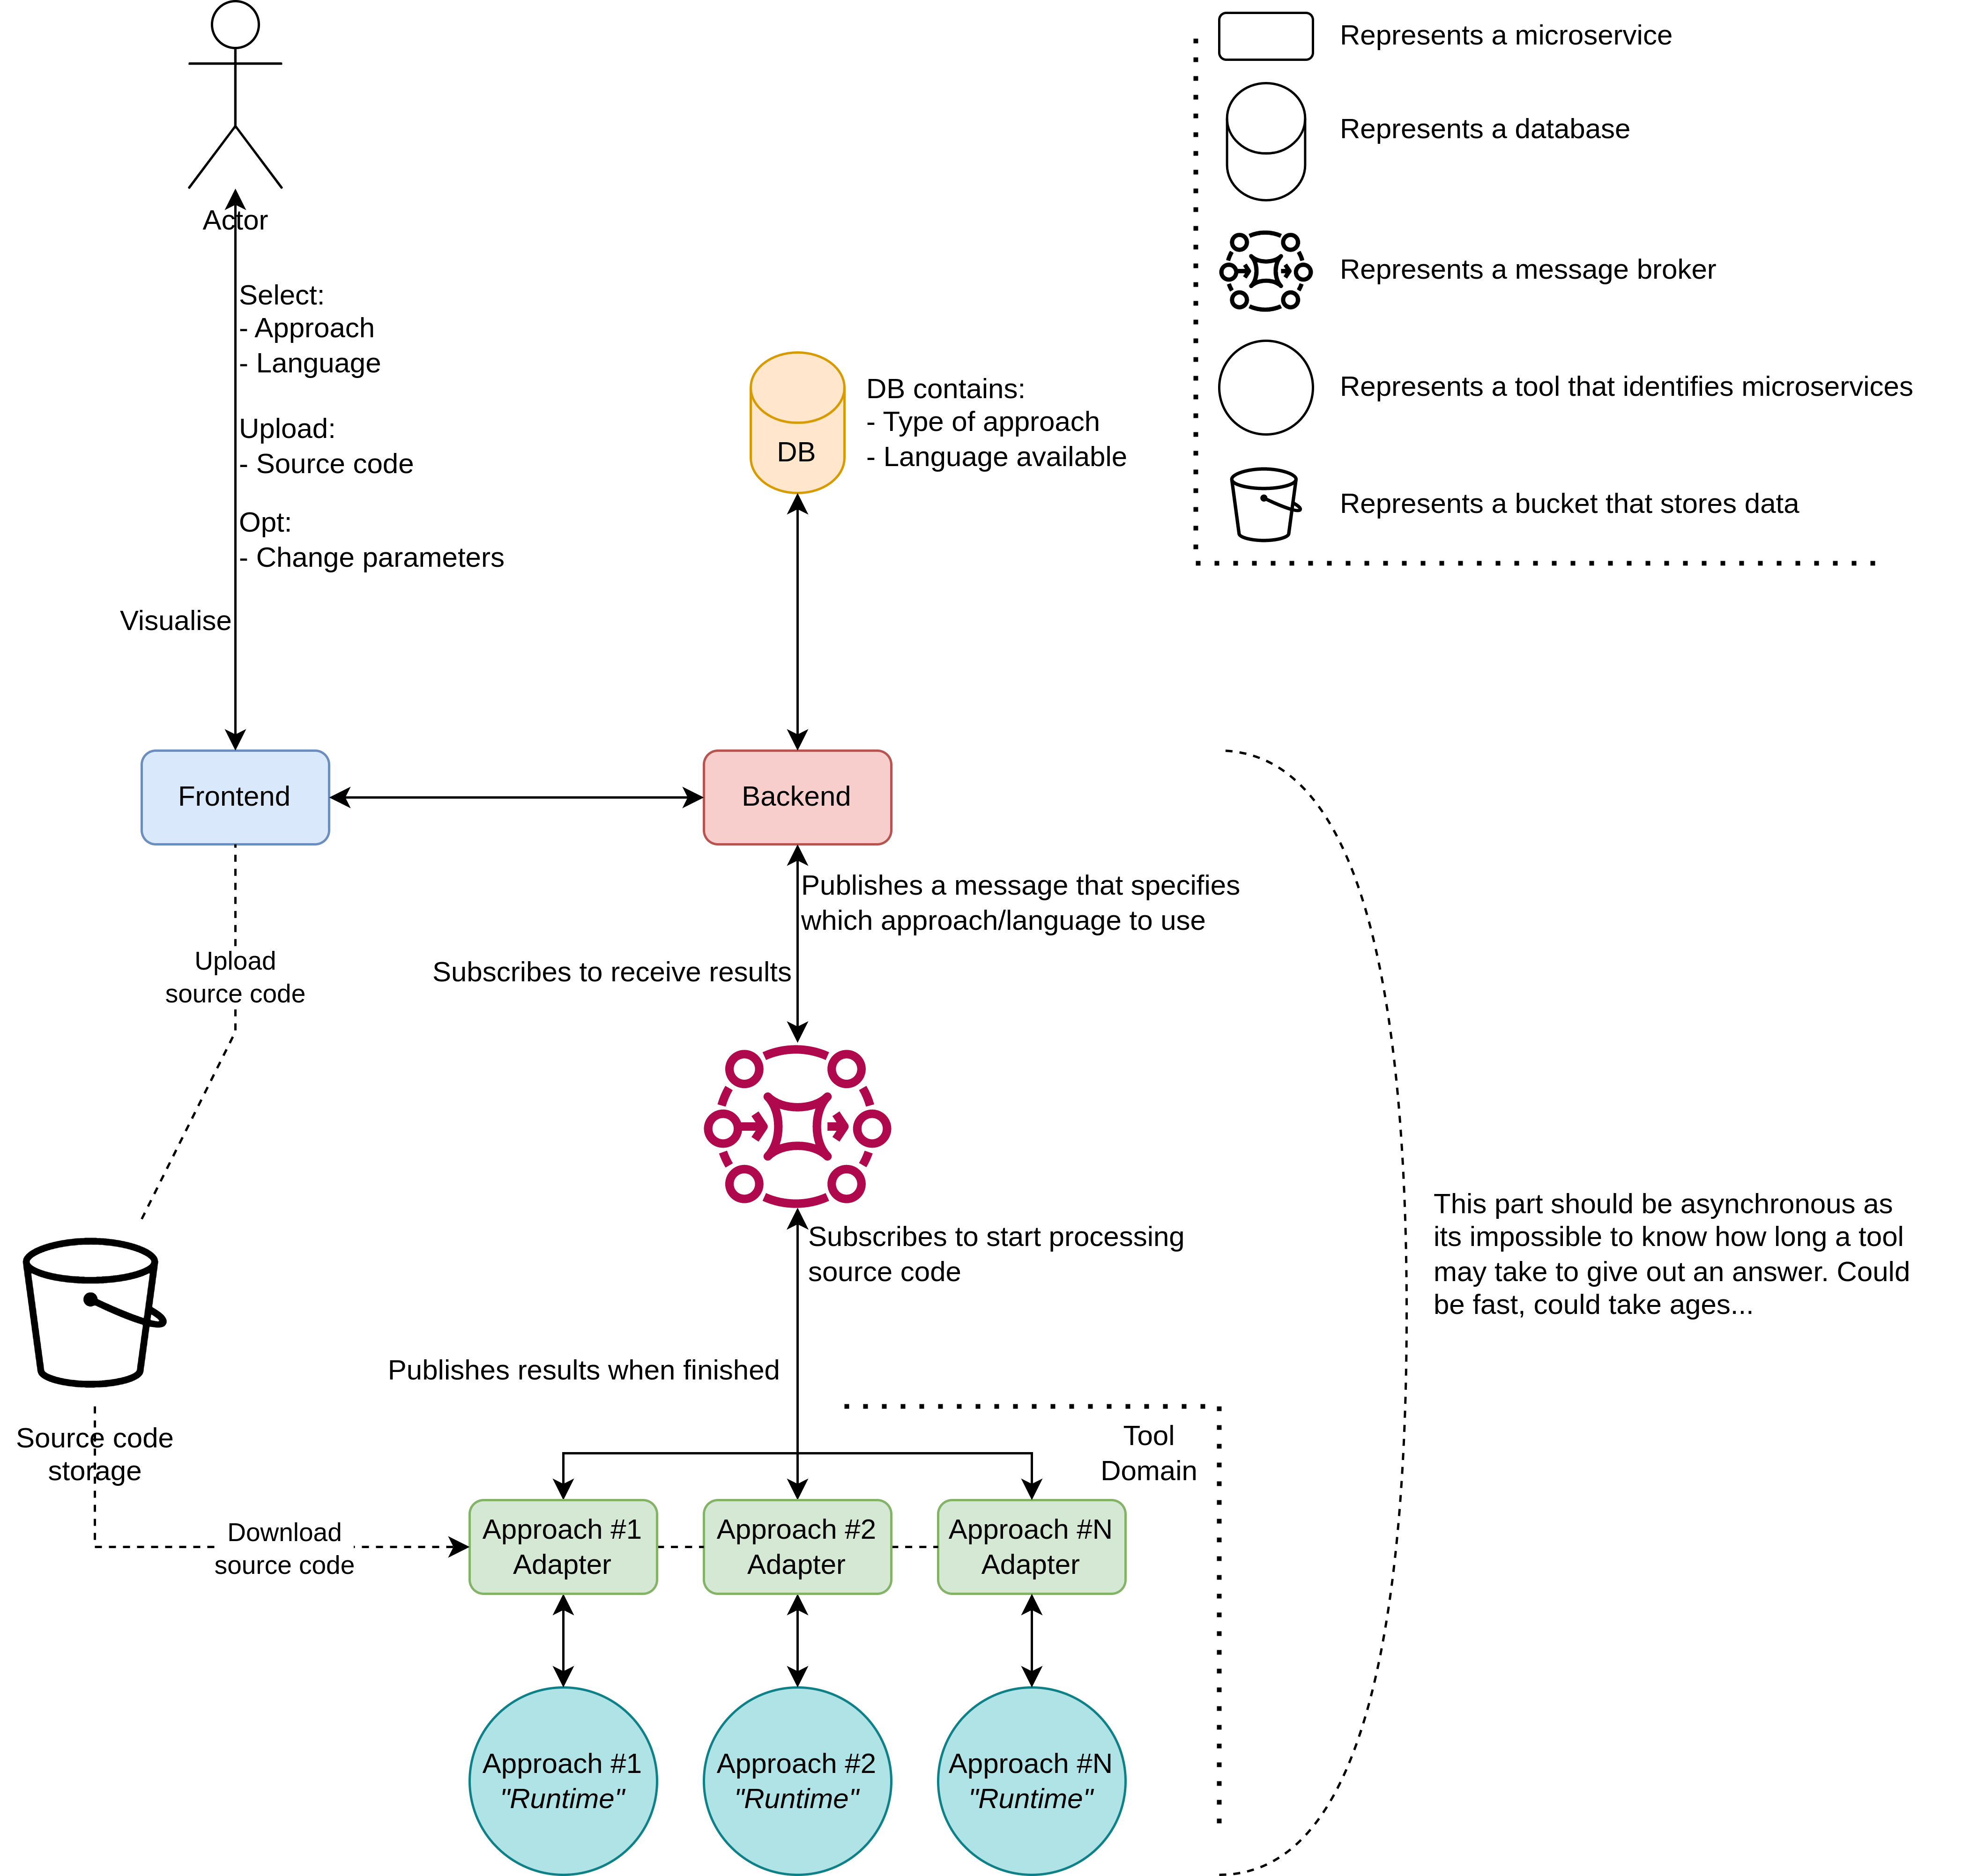
\includegraphics[width=\columnwidth]{thesis-architecture.drawio}
\end{figure}

The proposed tool architecture, as depicted in the sketch shown in Figure
\ref{fig:tool-architecture}, consists of three distinct components. The
frontend is responsible for the interface between the tool logic and the user.
The tools domain contains adapters for individual tools and the tool runtime,
which receives the monolithic input and generates the candidate microservices.
The backend serves as a bridge between the frontend, the database of available
tools, and the tools domain.

The main role of the backend component in the proposed tool architecture is to
initiate jobs and notify the frontend when a given job has completed. A job
consists of the process of identifying microservices from a given monolithic
input, which is then completed when the output containing the identified
microservices is produced. To avoid potential bottlenecks when multiple jobs
are run concurrently, the backend does not perform these tasks directly but
rather delegates them to the individual tools, therefore acting like a bridge.

The tools domain in the proposed tool architecture includes the tool runtime,
which contains the tool itself, and an adapter for the tool. The purpose of the
adapter is to provide a consistent interface for interacting with the tool,
regardless of the specific input and output formats that it uses. This is
important because different tools may accept different inputs and produce
different outputs, such as JSON or raw code. By using an adapter to translate
between these formats, it becomes easier to process the inputs and outputs of
the tool and integrate it with the overall tool logic. The tool runtime
receives the monolithic input and generates the candidate microservices, while
the adapter serves as a "middleman" between the tool runtime and the other
components of the architecture.

One of the first decisions that we have considered is which target platform the
tool should support. There are three major platforms that are relevant for this
purpose: macOS, Windows, and Linux. Determining which of these platforms to
focus on would require extensive surveying to ensure that the tool will be used
by the intended audience. While market share data suggests that Windows is the
most widely used desktop operating system, followed by macOS and Linux
\cite{desktop-usage-worldwide}, this may not necessarily reflect the operating
systems used by the architects, engineers, and developers who are responsible
for migration. Given the limited time frame, it is infeasible to conduct a
thorough survey to determine the preferred operating system of this target
audience. As a result, we have decided to adopt a more cross-platform solution.
After evaluating the options, we have determined that the browser is the most
suitable platform for this purpose.

Ideally, each component of the proposed tool architecture would be deployed as
a microservice in a Docker container to facilitate scalability and
cross-platform deployment. This is especially important for the tool runtime
component, as it is uncertain at this point whether the tools will take
advantage of multithreading. By using Docker, we can create a new container for
each job, which would allow us to handle multiple jobs concurrently and avoid
the need for users to wait for their jobs to complete. Of course, it is
possible that certain tool limitations may prevent us from implementing this
approach, but it is our goal to use microservices and Docker to the greatest
extent possible to ensure the flexibility and scalability of the tool.

Given that the tasks performed by the tool runtime component are asynchronous,
the communication between the tool runtime and the backend cannot be based on
synchronous HTTP request-response cycles. Instead, we will use a message queue
to connect the two components, with the use of message brokers. The backend
will send a message to initiate a job, which will be picked up by the
appropriate adapter and executed by the tool runtime. Once the job is
completed, the tool runtime will send another message to the backend to
indicate that it is finished. This approach allows us to process multiple jobs
concurrently and avoid potential bottlenecks in the communication between the
tool runtime and the backend.

\section{Conclusion and Future Work}

\bibliographystyle{unsrt}
\bibliography{IEEEfull,refs}

\bibliographystyleSLR{unsrt}
\bibliographySLR{IEEEfull,slr}

\end{document}
